\begin{frame}{Anticipatory reasoning}
\textbf{Objectives}:
\begin{itemize}
    \item Assess or reassess the feasibility of carrying out an activity
    \item Select the most relevant activity to be carried out
    \item Enrich and bring more precision to the agent's activity planning
\end{itemize}
\vspace{.3cm}
\par \textbf{Observation}: In most MAS anticipation approaches, the agents
\begin{itemize}
    \item can't get any information about what the other agents are planning to do
    \item are forced to try to predict what is going to happen in the future by performing microsimulations internally
\end{itemize}
\vspace{.3cm}
\par \textbf{Proposition}: Exploit the AGRET model
\begin{itemize}
    \item offers visibility on the future dimension of time
    \item take into account the three positions of time: past, present, and future. \alert{The consideration of the future position of time is original}
\end{itemize}

\note{
Maintenant que le support permettant l’échange d’informations sur les 3 dimensions : espace, temps et organisation est posé, je vais vous montrer comment nous l'exploitons afin d'enrichir les informations prises en compte dans le raisonnement anticipatif de l'agent. Les objectifs sont :
\begin{itemize}
    \item évaluer ou réévaluer la possibilité d'exécution d'une activité;
    \item choisir l'activité la plus pertinente à exécuter;
    \item enrichir et apporter plus de précision au planning d'activités de l'agent.
\end{itemize}
\par Pour se faire, nous exploitons AGRET et plus particulièrement la visibilité qu'il offre sur la position future du temps. Ces informations futures concernent les activités que les agents projettent d'effectuer. En effet, dans la plupart des approches d'anticipation dans les SMA, les agents sont contraints d'essayer de deviner ce qui va se passer dans le futur en réalisant des microsimulations en interne. Cela est dû au fait qu'ils ne peuvent avoir aucune information sur ce que les autres agents prévoient de faire. La mise en place de notre nouveau support qui est l'environnement temporel offre aux agents une visibilité sur cette dimension future du temps. 
\par Cette nouvelle dimension d'expression et de partage qui est de nature temporelle permet aux agents de partager leurs projets individuels et de les diffuser sur le collectif. L'analyse prédictive réalisée par les agents se base alors sur la perception de ce nouvel environnement commun, plutôt que par des calculs de simulation reproduits par chacun d'eux.
\par 
}
\end{frame}

\begin{frame}{Anticipatory reasoning}
\par \textbf{Method}
\begin{itemize}
    \item we consider that agents have a more or less defined activity schedule like in real life
    \item this schedule contains the past, present and future activities that the agent wishes to carry out
    \item this schedule is shared and made accessible by the agents at the level of the temporal environment, according to the rules of accessibility and the extent of the temporal horizon of perception of each agent or each type of agent
    \item We exploit this information that the agent can collect in the form of percepts at the level of the different environments of the system in order to question and improve each agent's activity planning
\end{itemize}
\par \textbf{Proposition} on 2 level
\begin{enumerate}
    \item \textbf{Agent level}: enrichment of the information taken into account at the level of the agent's anticipative reasoning: taking into account the future
    \item \textbf{Multi-agent level}: set up a notification system 
\end{enumerate}

\note{
Concrètement, nous considérons que les agents possèdent un planning d'activité plus ou moins défini comme dans la vie réelle. Ce planning rassemble les activités passées, présentes et futures que l'agent souhaite effectuer. Ce planning est partagé et rendu accessible par les agents au niveau de l'environnement temporel, en fonction des règles d'accessibilité et de l'étendue de l'horizon temporel de perception de chaque agent ou chaque type d'agent. Nous exploitons donc ces informations que l'agent peut récolter sous forme de percepts au niveau des différents environnements du système afin de remettre en question ce planning d'activité.
\par Pour mettre cela en place, nous proposons un ensemble de solution sur 2 niveaux : 
\begin{itemize}
    \item Au niveau de l'agent : nous enrichissons les informations prises en compte au niveau du raisonnement temporel en prenant en compte la dimension future du temps
    \item Afin d'articuler le niveau collectif, nous mettons en place au niveau multi-agents un système de notification
\end{itemize}
}
\end{frame}

\begin{frame}{Anticipatory reasoning}{Agent level}

A system composed of \textbf{3 models}
\begin{enumerate}
    \item A perception model
    \item A predictive model
    \item A decision model
\end{enumerate}
\begin{figure}
	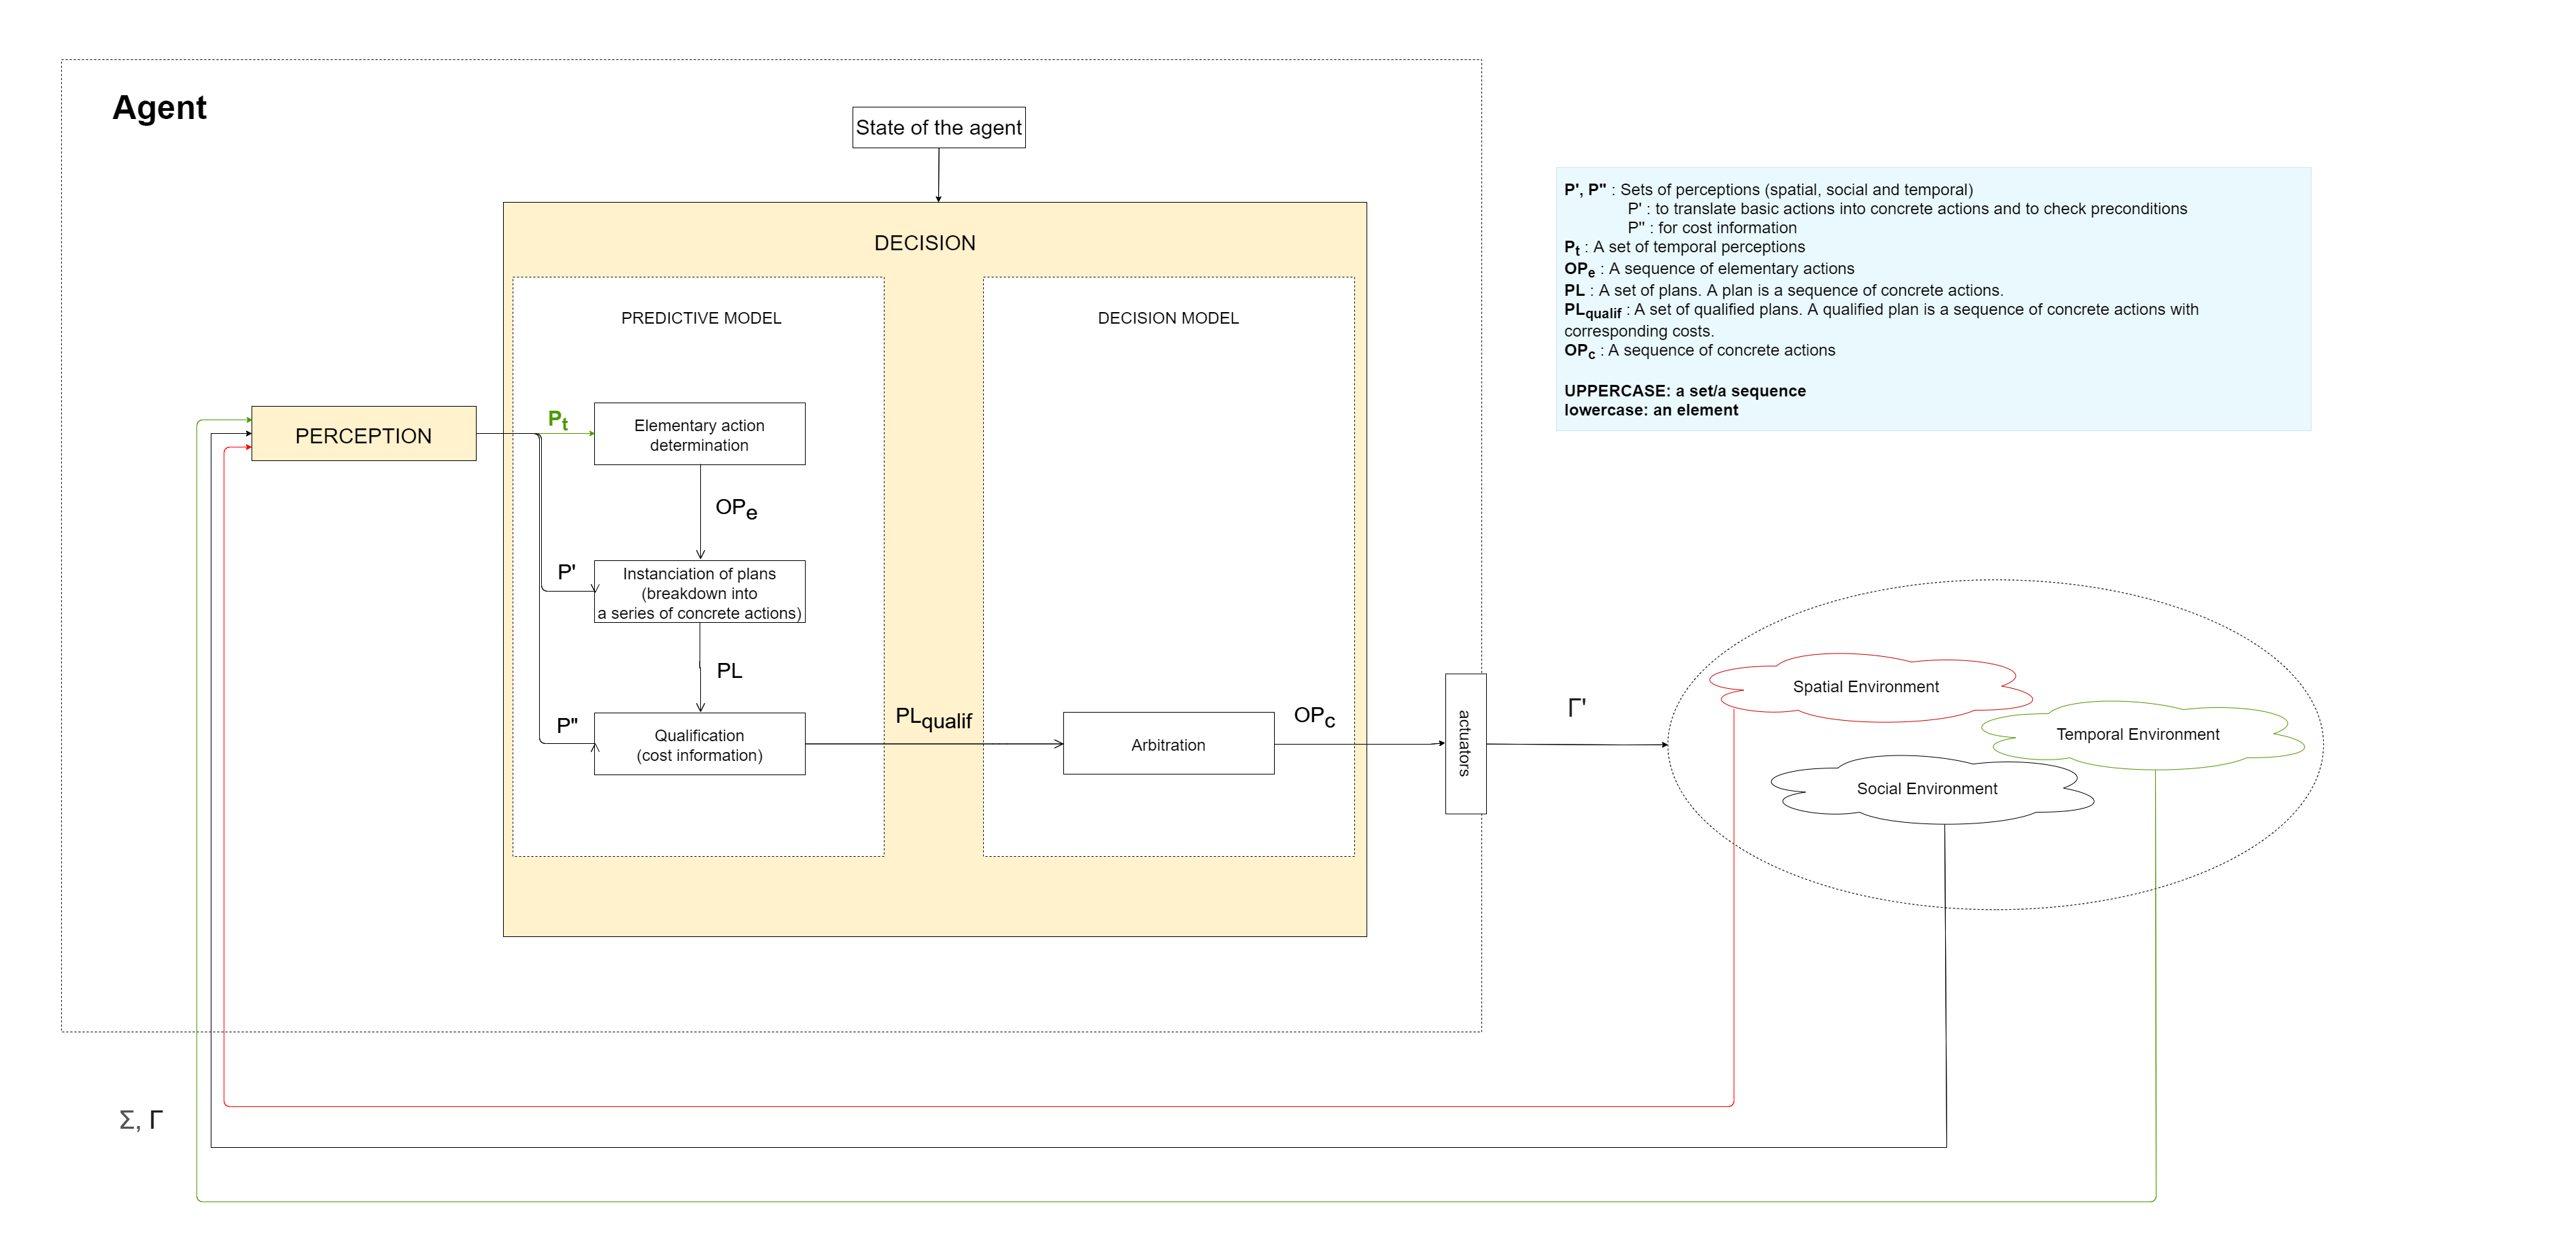
\includegraphics[width=.9\textwidth]{figures/Anticipation_english.png}
\end{figure}

\note{
\par Notre modèle d’agent se compose de 3 modèles:
\begin{enumerate}
    \item Un modèle de perception
    \item Un modèle prédictif
    \item Un modèle de décision
\end{enumerate}
Nous allons détailler le fonctionnement de chacun de ces modèles dans la suite de cette présentation
}
\end{frame}

\begin{frame}{Agent level}{Perception Model}
\par Perception of the agent spatial, social and temporal context
\par \extbf{Constraints}:
\begin{itemize}
    \item At the agent level: perception time window
    \item At the environment level: accessibility rules, storage time window
\end{itemize}
\par Similar to shared information sources checking we do in real life. Ex: agenda, schedule, social networks, etc.

\begin{equation*}
     Perception:\underbrace{\footnote{environment state}\Sigma_t \times \footnote{perception window}\Delta_{pt}}_{time} \times \underbrace{\Sigma_e \times \Delta_{pe}}_{space} \times \underbrace{\Sigma_s \times \Delta_{ps}}_{organisation} \times \footnote{influence}\Gamma \mapsto P
\end{equation*}
\note{
La perception permet à l’agent de prendre en compte les informations concernant son contexte d’activation. La mise en place de AGRET dans notre système permet à l’agent de percevoir son contexte spatial, social et temporel. Dans la pratique, les percepts temporels permettent à l’agent de prendre connaissance de l’ensemble des activités qu’il prévoit d’effectuer à l’instant présent. En fonction de l’étendue de son horizon temporel de perception, il peut également percevoir, l’ensemble des activités qu’il projette d’effectuer dans le futur ou qu’il avait prévu d’effectuer dans le passé. En fonction des règles d’accessibilité, l’agent peut également percevoir des informations concernant la dynamique temporelle des autres agents, que ces derniers partagent au niveau de l’environnement temporel. Ces informations temporelles captées par l’agent découlent des localisations temporelles que chaque agent du système a définies et partagées au niveau de l’environnement temporel. Dans la réalité, ce fonctionnement est similaire à la consultation d’un agenda privé ou partagé, d’un emploi du temps, ou de différentes sources
d’informations partagées comme les réseaux sociaux, par un agent, avant d’effectuer une action ou avant de planifier une future action.
\par Dans IRM4S, la contrainte par un ou plusieurs horizons de perception n'est pas explicitement affichée dans la formule correspondante à la perception. Contrairement à cela, dans notre approche, nous distinguons clairement les horizons de perception : temporel, spatial et social en les rajoutant explicitement dans la description formelle du fonctionnement du module perception. Ces horizons contraignent la perception de l'agent. Les percepts générés en sortie sont alors un ensemble de trois types de percepts différents, mais complémentaires : temporels, spatiaux et sociaux.

}    
\end{frame}

\begin{frame}{Agent level}{Predictive Model}
\begin{block}{Action Model}
\par Features : 
\begin{itemize}
    \item Preconditions
    \item Costs. Ex: energy, queuing, etc.
    \item Influence
    \item Corresponding actuators
\end{itemize}
\vspace{.3cm}
\par 2 types of actions:
\begin{itemize}
    \item elementary action: abstract. Ex: go to work, go to play
    \item concrete action: located. Ex: go to work at the 8:00 A.M. (time location) at the university (space location)
\end{itemize}
\end{block}
\begin{block}{Environment model}
\end{block}

\note{
\footnotesize{
Certaines approches d'anticipation dans les SMA reposent sur la capacité des agents à réaliser des prédictions. Grâce à ces prédictions, l’agent peut s’attendre à la réalisation d’événements futurs, et agir au préalable. Le modèle prédictif prend en compte le contexte d'activation temporel, spatial et social des agents et génère des instanciations de plans d'actions et une estimation de leurs coûts. 
Ce modèle se compose généralement
d’un modèle d’action d’un modèle de l’environnement. Le modèle d’action que nous utilisons est classique. Une action est caractérisée par :
\begin{itemize}
    \item Un ensemble de préconditions qui doivent être remplies  pour que l’action puisse être réalisée. Les préconditions permettent le chaînage des actions en vue de réaliser un but. Si un agent veut obtenir les effets d’une action, mais que les préconditions de cette action ne sont pas remplies, il va chercher un ensemble d’autres actions à effectuer au préalable, et ainsi de suite.
    \item Une influence sur l’agent et/ou sur l’environnement
    \item Des coûts : Nous partons du principe selon lequel les actions peuvent avoir des importances et rôles différents selon les simulations. Nous laissons donc la possibilité au modélisateur de rajouter des critères de coût sur les actions.
    \item Des actionneurs correspondant
\end{itemize}
\par Nous distinguons notamment deux types d’actions:
\begin{itemize}
    \item les actions e qui correspondent à des opérateurs relatifs à une activité. Une action élémentaire est abstraite.
    \item les actions c : instanciation d’une action e dans l'environnement. En d'autres termes la prise en compte de la réalité environnementale concrète dans une action abstraite. Une action concrète est située.
\end{itemize}
}}
    
\end{frame}

\begin{frame}{Agent level}{Predictive Model}
\begin{block}{Action Model}
\end{block}
\begin{block}{Environment Model}
\par \textbf{In classical approaches}: Accelerated simulation of the representation of the environment within the agent himself. It expresses
\begin{itemize}
    \item probabilities of occurrence of events conditioned by the time of the simulation or by the triggering of other events
    \item general facts about the world (locations, opening hours, weather conditions, etc.)
    \item approximations of travel time
\end{itemize}
\medbreak
\par \textbf{In our approach}: generates a set of possible activity plans with their costs
\vspace{.5cm}
\par \textbf{Proposition}: \st{Accelerated simulation of the representation of the environment within the agent himself}
\medbreak
The future state of the world is constructed from the perception of the temporal environment

\end{block}

\note{
\footnotesize{
Maintenant parlons du modèle d’environnement:
En tant qu'humains, nous effectuons des prédictions de manière très naturelle, sans en avoir réellement conscience. Cependant, pour qu’un agent puisse anticiper, même des événements qui peuvent paraître évidents, il est indispensable que ces  derniers soient mentionnés dans le modèle de l’environnement. Dans les approches classiques, ce modèle est capable d’exprimer, par exemple :
des probabilités d’apparition d’événements conditionnées par l’heure de la simulation ou par le déclenchement d’autres événements;
des faits généraux sur le monde (lieux, horaires d’ouverture, conditions météo, etc.);
Des approximations de temps de trajet.
\par Dans notre cas, elle permet d'enrichir cela par la prédiction d'un ensemble de plan d'activité possible. Dans certaines approches, le fonctionnement d'un tel modèle consiste à simuler en accéléré la représentation de l’environnement au sein même de l'agent et ainsi fournir des prédictions.  L'approche que nous proposons est différente de cela car nous construisons différemment nos prédictions externes, c'est-à-dire l'état futur du monde. Notre modèle d'environnement temporel, diffère des modèles classiques :  il est construit à partir de la perception de l'environnement temporel. Plus particulièrement, nous exploitons la perception de la dimension future du temps qui résulte des informations que les agents partagent sous forme de localisations temporelles au niveau de l'environnement temporel. Une partie de l'état prévisionnel du monde est donc obtenu par perception de l'axe temporel prévisionnel contenu dans l'environnement temporel et qui a été illustré par le schéma que j’ai expliqué précédemment. \par Cet axe est alimenté et mis à jour par les agents eux-mêmes. Cela nous permet de nous affranchir des approches classiques qui réalisent, au sein même de chaque agent, des microsimulations pour générer des prédictions. }}
\end{frame}

\begin{frame}{Agent level}{Predictive Model}
\par Composed of 3 blocks
\begin{itemize}
    \item Determination of elementary actions: generates a sequence of elementary actions to be carried out taking into account all temporal perceptions.
    \item Instanciation of plans \footnote{We can plan $OPc$, a sequence of concrete actions $OPc = \{opc_{1}, opc_{2}, ... , opc_{n} \}$}
    \begin{itemize}
        \item situation of an elementary action (declination into concrete actions)
        \item verification of preconditions
    \end{itemize}
    \item Qualification : cost information
\end{itemize}
\par \textbf{Input}: set of spatial, social and temporal perceptions
\par \textbf{Output}: 
A set of concrete action plans with the costs corresponding to each action. Example:
\begin{itemize}
    \item the expected queue length $q_0$
    \item the expected energy cost $e$
    \item the criticality $cr$ (the degree of importance that the agent gives to an action)
\end{itemize}


\note{

Notre modèle prédictif est constitué de trois blocs :
\begin{itemize}
    \item la détermination d’actions élémentaires qui permet à l’agent de générer un enchaînement d’actions élémentaires à réaliser en tenant compte de l’ensemble des percepts temporels qu’il reçoit du module perception et de son état interne. Pour ce faire, il fait correspondre une action élémentaire à une localisation temporelle, selon les informations contenues dans cette dernière.
    \item L’instanciation de plans qui consiste en l’exécution de deux processus : la situation d’une action élémentaire au niveau des environnements (déclinaison en actions concrètes)
    \item La vérification de l’applicabilité d’une action concrète (vérification des préconditions). Cette étape consiste à renseigner l’ensemble des coûts correspondant à chaque déclinaison d’action concrète.
\end{itemize}
Le modèle prédictif prend donc en entrée un ensemble de percepts spatiaux, sociaux et temporels. Il génère à sa sortie un ensemble de déclinaisons de plans d’actions concrètes avec les coûts correspondants à chaque action.
Ces coûts peuvent être par exemple: le coût associé la longueur prévisionnelle de la file d’attente q0 ; le coût énergétique e, la criticité cr (le degré d’importance que l’agent accorde à une action). Plus la valeur de la criticité se rapproche de 0, moins l’agent accorde de l’importance à l’action associée. Contrairement à cela, plus la valeur de la criticité se rapproche de 1, plus l’agent considère l’action comme importante.


}
    
\end{frame}

\begin{frame}{Agent level}{Decision Model}
The decision model:
\begin{itemize}
    \item Includes only an arbitration module 
    \item Proposes a behaviour or action based on the predictions generated by the predictive model
    \item Selects the most relevant plan based on a minimization of weighted costs
\end{itemize}

\vspace{.5cm}
\par Each action that composes the plan is sent to the actuators to be transformed into influences:
    \begin{itemize}
        \item Actions that must be executed immediately are sent to the corresponding actuators
        \item Actions to be executed later are sent to the temporal environment actuators to be transformed into temporal locations. In this way, the agent obtains a richer and more precise activity schedule
    \end{itemize}


\note{
Comme dans un modèle d’agent classique intégrant un raisonnement anticipatif, le modèle de décision propose un comportement ou une action à partir des prédictions générées par le modèle prédictif. Notre modèle de décision procède à la sélection du plan le plus pertinent. Cette sélection s'appuie sur une minimisation des coûts pondérés. En d'autres termes, le plan le plus pertinent est celui dont la somme des coûts pondérés des actions qui le composent est minimale.
\par Le modèle de décision comprend uniquement un module d’arbitrage. Son fonctionnement consiste en une comparaison des instanciations de plan sur la base des coûts correspondants. Notre module décisionnel exploite donc les informations collectées à travers les perceptions spatiale, temporelle et sociale traduites sous forme de coûts par notre modèle prédictif pour l’arbitrage des décisions. Pour ce faire,  il applique une pondération sur chaque coût correspondant à chaque action composant le plan. Le choix repose sur la minimisation des coûts pondérés. Les valeurs des pondérations sont arbitraires. Elles sont définies par le concepteur du modèle ou par l’utilisateur en fonction des objectifs de la simulation. 

Une fois l’instance de plan de coût pondéré minimale choisit, chaque action le composant est envoyée aux actionneurs pour être transformée en influences. Les actions qui doivent être immédiatement exécutées sont envoyées aux actionneurs correspondants. Les actions qui doivent être exécutées plus tard quant à elles sont envoyées aux actionneurs de l’environnement temporel afin qu’elles puissent être transformées en localisations temporelles. De cette manière, l’agent obtient un planning d’activités plus riche et plus précis.


}
    
\end{frame}

\begin{frame}{Multi-agent level}
\par \textbf{Proposition}: A notification system
\begin{itemize}
    \item the agent is notified of events that may affect the execution of an action that it has planned
    \item the agent may then be led to question his wish to carry out this action
\end{itemize}

\par \textbf{Method}:
\begin{itemize}
    \item  The agent programs itself its activation by defining a temporal location in the temporal environment
    \item We influence its behaviour by means of a notification. The aim is to encourage the agent to question its decision.
\end{itemize}

\note{
Comme préciser au tout début de la présentation, notre cadre applicatif qui est le concept de ville intelligente implique le choix d'une approche ascendante, distribué. Une forme d'intelligence participative où chaque entité du système agit de manière pro-active pour la satisfaction d'un objectif en commun. Ainsi, afin d'articuler le niveau multi-agents, nous mettons en place un système de notification. Dans l'approche d'anticipation que nous proposons, l'agent peut être notifié des événements pouvant avoir des conséquences sur l'exécution d'une action qu'il a planifiée dans le futur (sous forme de localisation temporelle). Il peut alors être amené à remettre en question son souhait d'exécution de cette action.
\par En effet, l'agent programme lui même son activation en définissant une localisation temporelle au niveau de l'environnement temporel. Cependant, il est possible d'influencer son comportement par le biais d'une notification. Il peut donc être amené à remettre en question sa décision suite à la réception d'une notification due à un changement au niveau de l'environnement.
\par Dans l'approche d'anticipation que nous proposons, l'agent peut être notifié des événements pouvant avoir des conséquences sur l'exécution d'une action qu'il a planifiée dans le futur (sous forme de localisation temporelle). Il peut alors être amené à remettre en question son souhait d'exécution de cette action. Ces événements concernent la création, la suppression, ou la modification d'une ou d'un ensemble de locations temporelles par d'autres agents. 

}
    
\end{frame}

\begin{frame}{Multi-agent level}
\par \textbf{Set-up}:
\begin{itemize}
    \item By default by the system designer. Example: based on spatial distance
    \item Voluntarily by agents by subscribing to a particular object in the environment Example: a temporal slot, a charging point
\end{itemize}
\vspace{.3cm}
\begin{columns}
\begin{column}{.45\linewidth}
\begin{figure}
	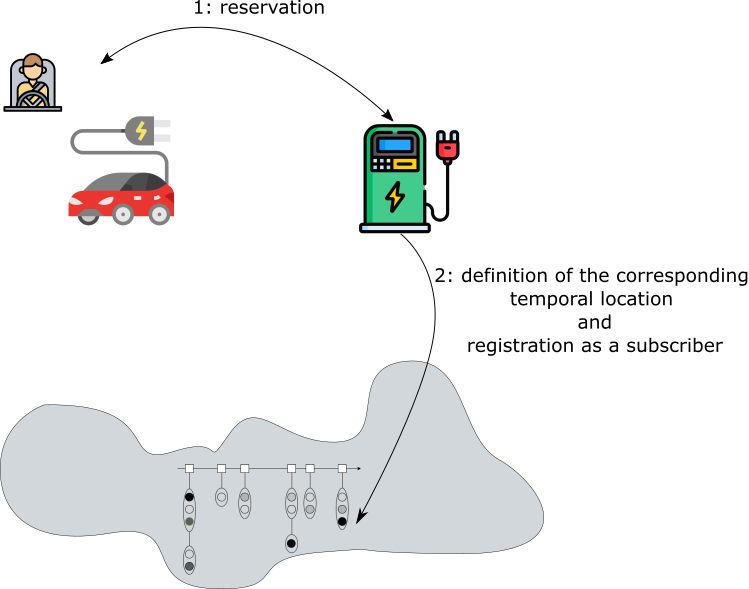
\includegraphics[width=\textwidth]{figures/example1.png}
\end{figure}
\end{column}
\begin{column}{.55\linewidth}
\begin{figure}
	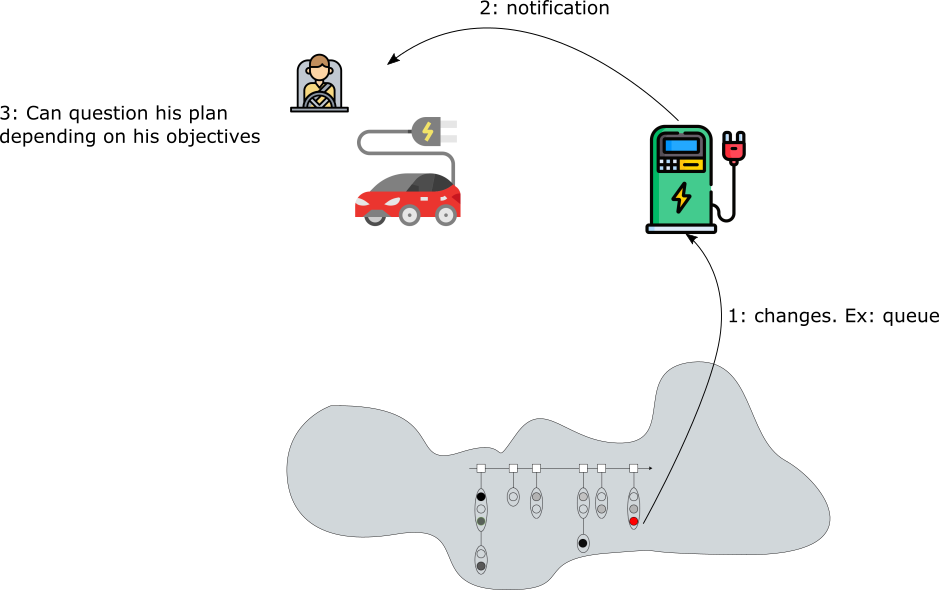
\includegraphics[width=\textwidth]{figures/example2.png}
\end{figure}
\end{column}
\end{columns}

\note{
Cette fonctionnalité peut être mise en place et activée de deux manière:
\begin{itemize}
    \item par défaut par le concepteur du système
    \item volontairement par les agents, sous forme d'abonnement à un slot particulier de l'environnement temporel ou à un objet particulier de l'environnement spatial comme une borne de recharge par exemple.
\end{itemize}
 Dans notre modèle de simulation, lorsqu'un automobiliste réserve une borne, la borne définit une localisation temporelle qui traduit sa volonté de recharger le véhicule à un instant $t$. Dans ce cadre, elle inscrit automatiquement l'automobiliste en tant qu'abonné aux mises à jour concernant les modifications de cette localisation temporelle.  Ainsi, l'automobiliste est tenu au courant, par exemple, d'un changement au niveau de la longueur prévisionnelle de la file d'attente. Il peut par la suite remettre en question son action de se recharger sur cette borne à cet instant. En fonction de ses objectifs, si l'agent suppose que la file d'attente est trop longue, il peut relancer son processus de raisonnement afin de rechercher une autre borne de recharge ou un autre créneau qui lui convienne mieux.
    
    }
\end{frame}

\begin{frame}{Multi-agent level}
\par \textbf{Set-up}:
\begin{itemize}
    \item By default by the system designer. Example: based on spatial distance
    \item Voluntarily by agents by subscribing to a particular object in the environment Example: a temporal slot, a charging point
\end{itemize}
\vspace{.3cm}
\begin{figure}
	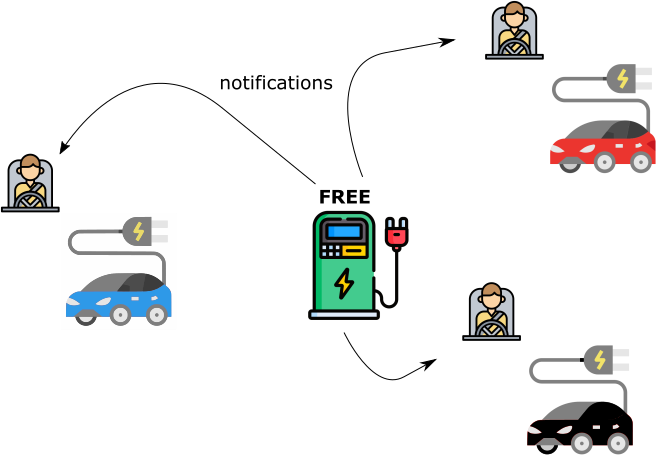
\includegraphics[width=.55\textwidth]{figures/example3.png}
\end{figure}
\note{
 Un autre fonctionnement de ce processus de notification consiste à alerter tous les agents à proximité lorsqu'une borne de recharge est disponible. 
    
    }
\end{frame}

\begin{frame}{Implementation}

    \begin{figure}
	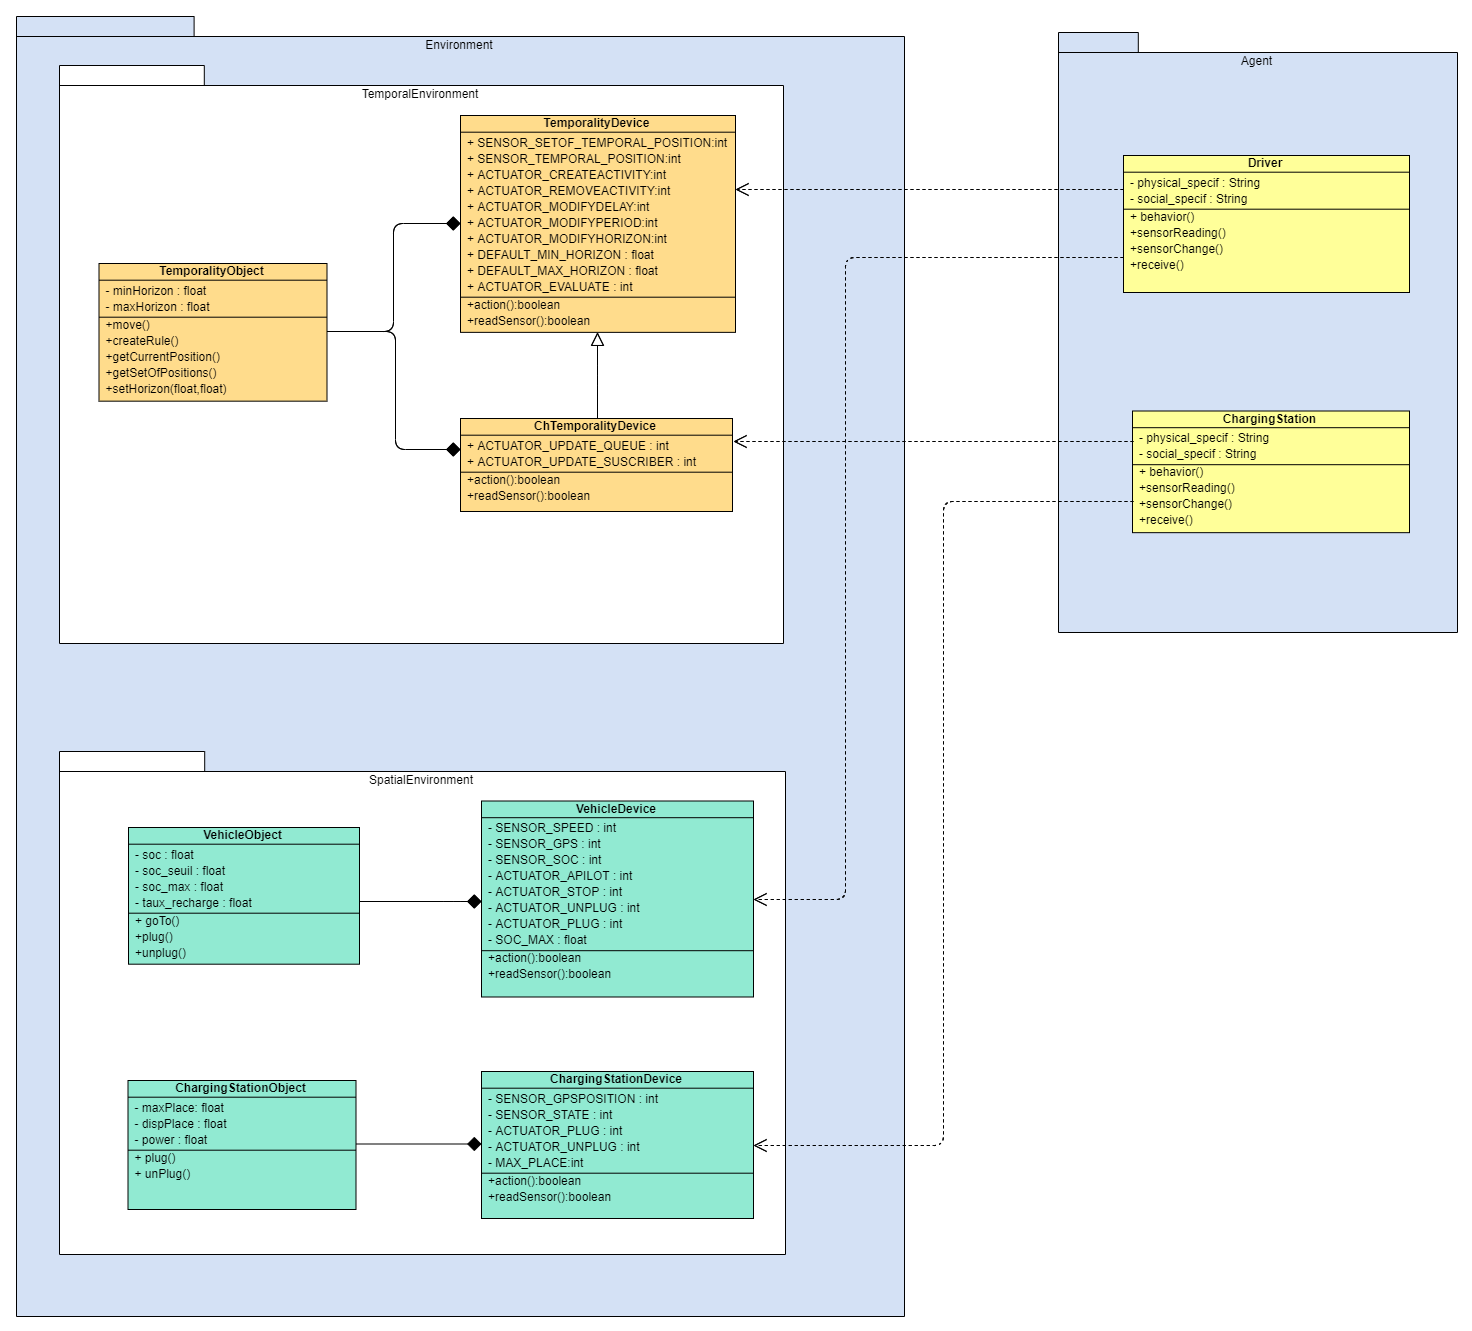
\includegraphics[width=.65\textwidth]{figures/Agent_Environnement_SkuadCityModel.png}
	\end{figure}
    
\note{
Le diagramme UML suivant montre un exemple d'implémentation de notre deuxième contribution dans le cadre de l’exemple du rechargement de véhicules électrique avec des bornes de recharges publiques. 
La mise en oeuvre du raisonnement anticipatif se fait uniquement au niveau de l’agent, aucune implémentation n’est alors effectué au niveau de la plateforme de simulation.
Cette mise en oeuvre met en jeu les deux environnements physiques :
\begin{itemize}
    \item L’environnement spatial et l’environnement temporel où nous pouvons voir clairement sur le schéma les représentations de l’agent dans chaque environnement
    \item L’environnement social donc le câblage se fait par la spécification du slot social “social\_specif”
\end{itemize}
}
\end{frame}

\begin{frame}{Implementation}
\begin{figure}
	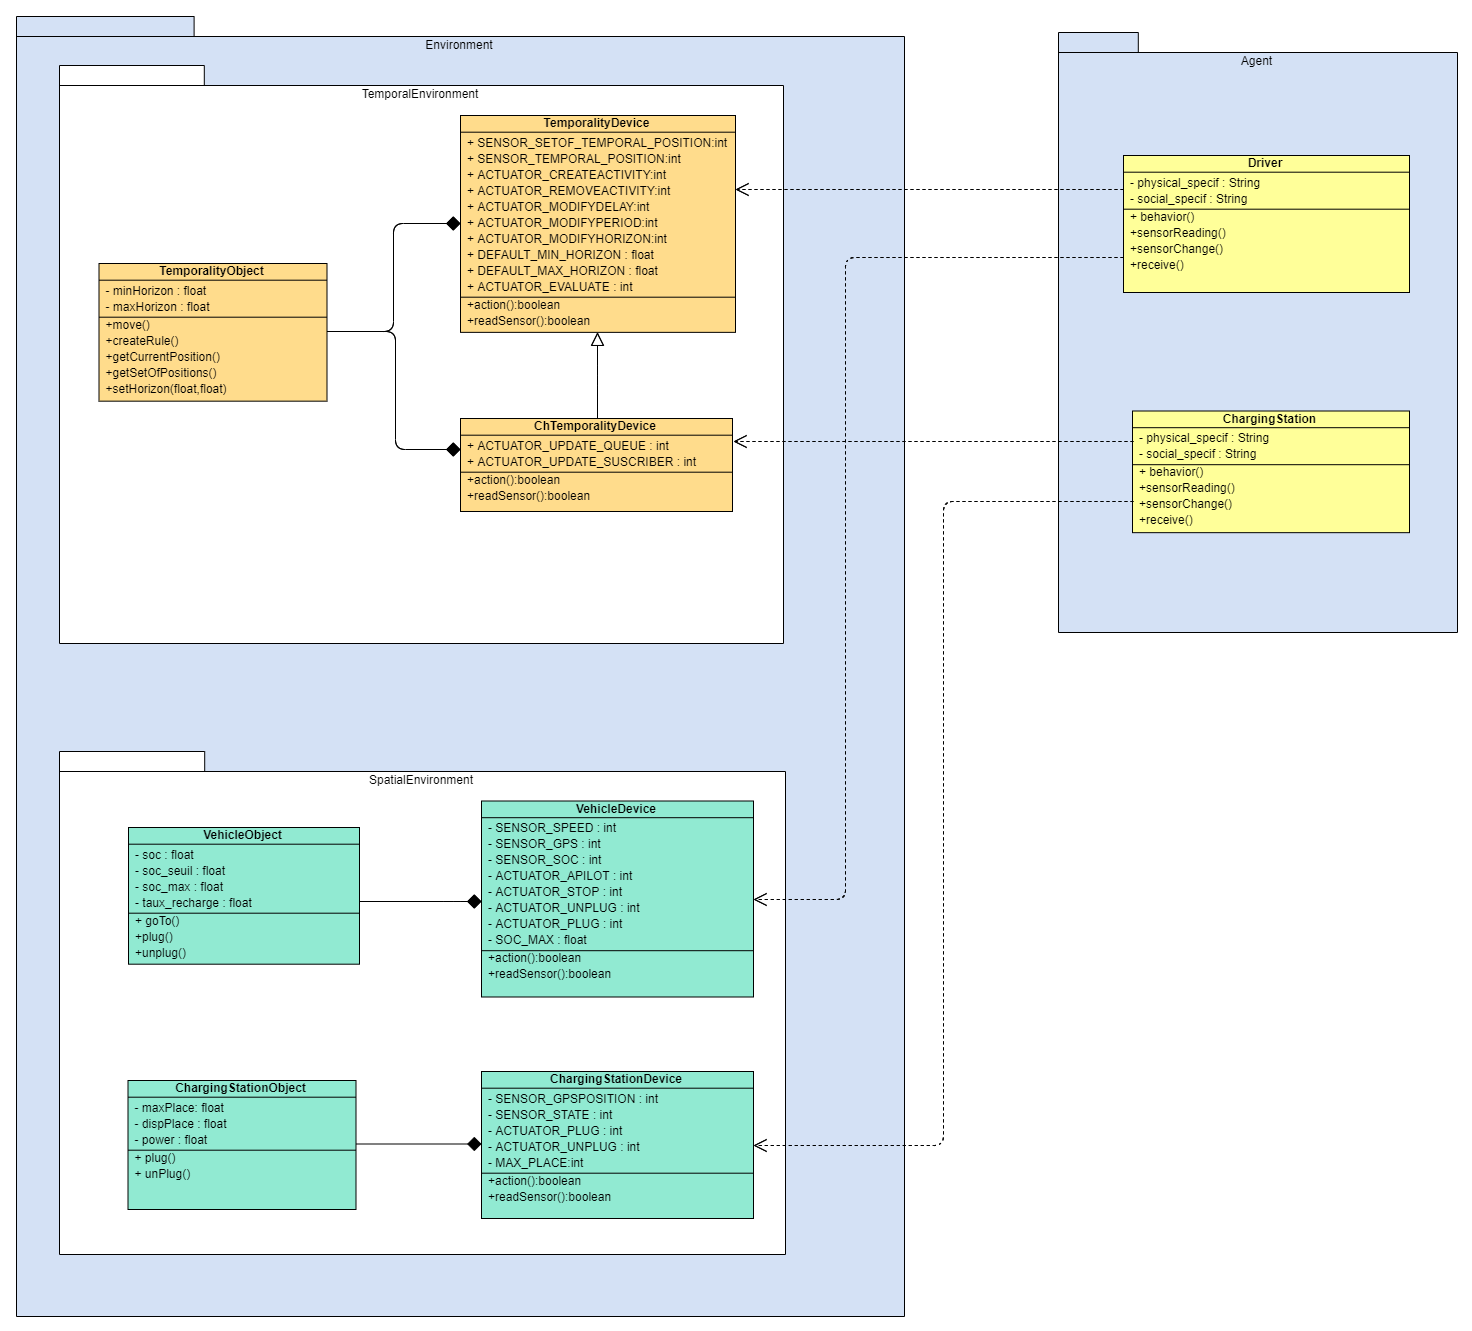
\includegraphics[width=.65\textwidth]{figures/Agent_Environnement_SkuadCityModel.png}
\end{figure}
\note{
Dans notre scénario nous en rajoutons 3 paramètres optionnels à une localisation temporelle: l'appréciation, la longueur prévisionnelle de la file d'attente et la liste des abonnés. L’appréciation indique pour chaque action passée le niveau de satisfaction global d’un agent par rapport à l'exécution de l'action. Ce niveau de satisfaction est stocké au niveau de la localisation temporelle correspondante. Ce paramètre se renseigne uniquement sur des localisations temporelles passées. Il s'agit d'ailleurs, dans notre cas, de la seule modification qu'un agent peut effectuer sur une localisation temporelle passée. Nous avons choisi une notation simple 0 ou 1. 1 pour dire que l'action a bien été exécutée et 0 si elle n'a pas pu être exécutée. Cependant, il est tout à fait envisageable de définir un système de notation plus détaillé avec des valeurs variant entre 0 et 1. L'appréciation et la liste des abonnés sont des paramètres génériques qui peuvent être réutilisés dans n'importe quel autre modèle de simulations. Par contre, la longueur prévisionnelle de la file d'attente est un paramètre optionnel propre à la gestion de ressource partagée et limitée dans le temps et de l'espace. Sa pertinence dépend donc du contexte applicatif. Ces paramètres facultatifs servent à renseigner le coût des actions et à améliorer l'arbitrage de la décision au niveau du raisonnement anticipatif. Par défaut, ces paramètres prennent une valeur nulle. 
}
    
\end{frame}

\begin{frame}{Implementation}
\begin{figure}
	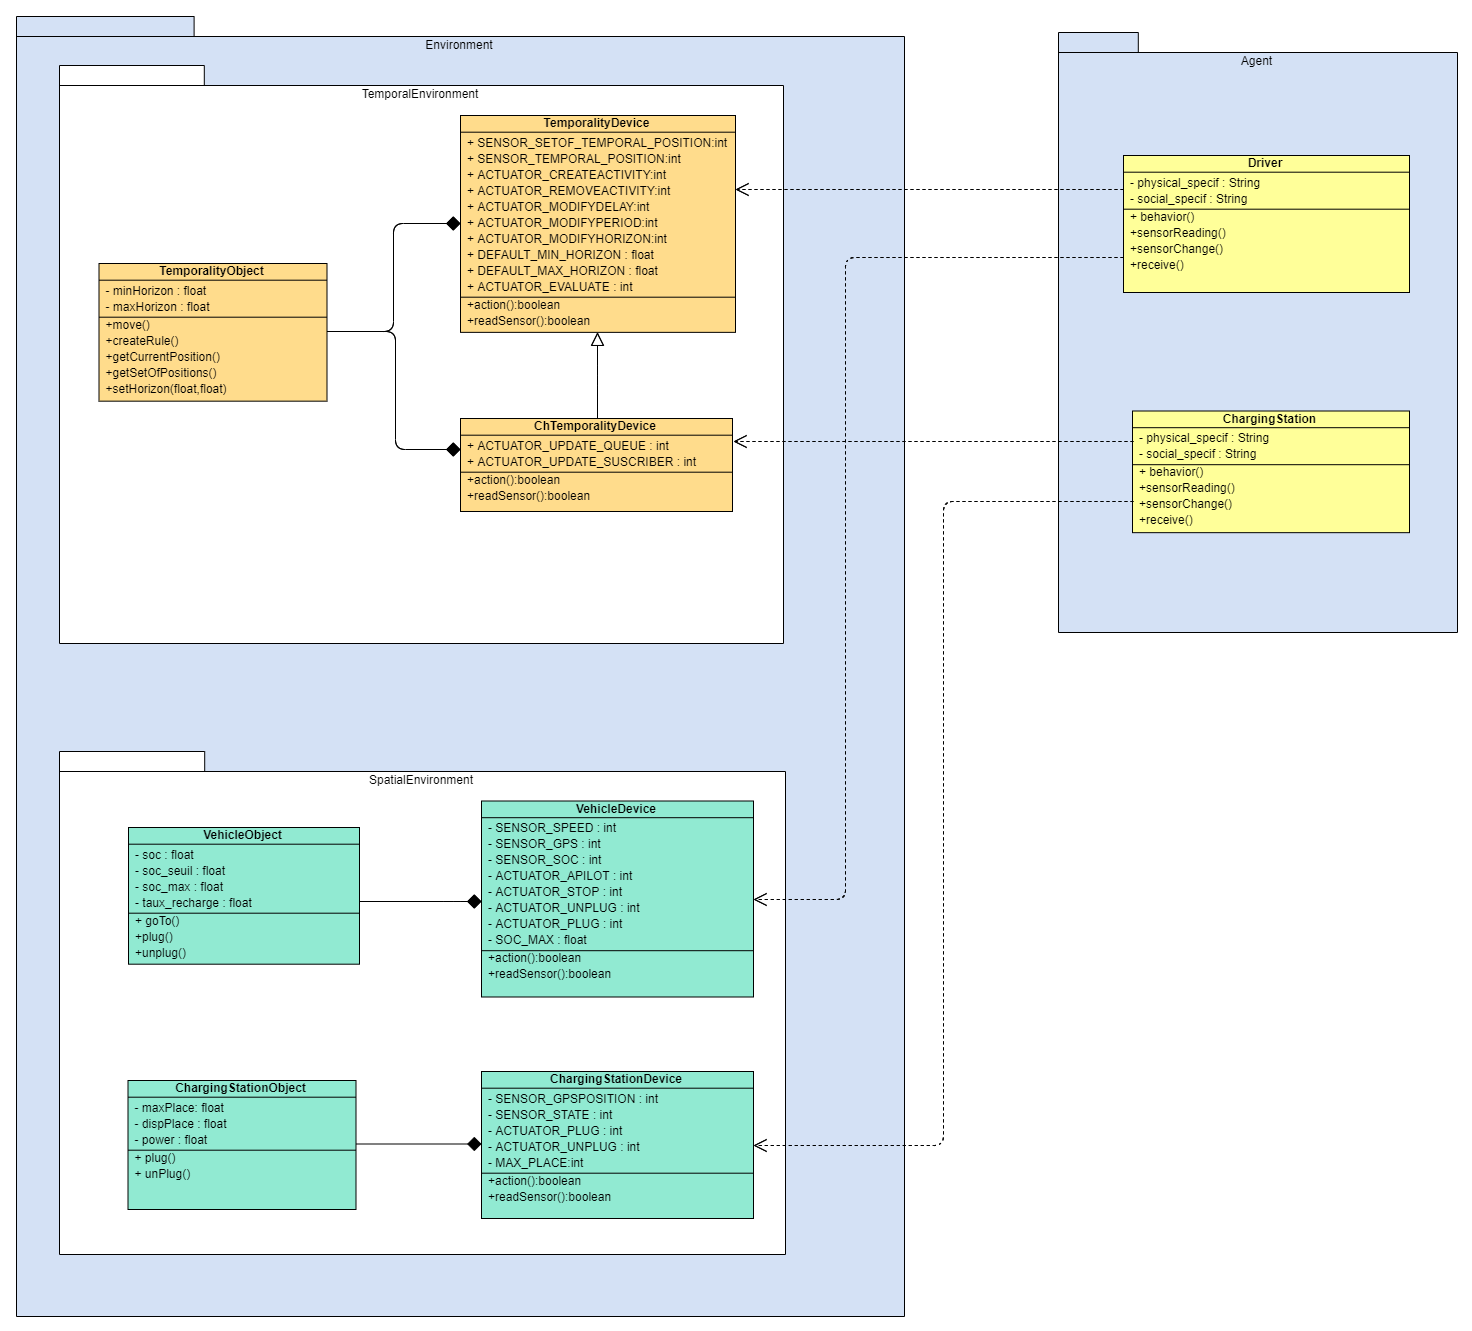
\includegraphics[width=.65\textwidth]{figures/Agent_Environnement_SkuadCityModel.png}
\end{figure}

\note{

\par \textbf{Mise en oeuvre de la perception}:
Dans SkuadCityModel, la perception des informations au niveau des environnements physiques se fait par le biais des capteurs intégrés dans les devices VehicleDevice et TemporalityDevice. La méthode correspondante est la méthode readSensor. Le recueil des informations au niveau de la dimension sociale quant à lui s'effectue par lecture de message par le biais du système de boîte mail. La méthode correspondante est la méthode receive.
Plus particulièrement, au niveau de l'environnement temporel, comme nous l'avons expliqué, la perception se fait par le biais des capteurs: SENSOR\_TEMPORAL\_POSITION et SENSOR\_SETOF\_TEMPORAL\_POSITION. 
\par \textbf{Mise en oeuvre du modèle prédictif}: La plupart des méthodes relatives à l’implémentation de ce modèle prédictif sont intégrés au niveau de la classe Driver: generateConcreteActionList(), situate(), checkApplicability(), plan (), checkForPriorAction(), qualify(),...
\par \textbf{Mise en oeuvre du modèle de décision}: Les méthodes qui entrent en jeu sont weight() et choose()
}
\end{frame}